\documentclass{article}
\usepackage{amsmath}
\usepackage{listings}
\usepackage{xcolor}
\usepackage{graphicx}
\usepackage[margin=1in]{geometry}


\title{Solving the HJB Equation of the Huggett Model\\[5pt] {\Large \textbf{Coding Homework \#3}}}

\author{Rafael Pintro Schmitt}

\date{}

\begin{document}

\maketitle 

\subsection*{Question 1}
As seen in the plot, consumption for both the employed and unemployed is increasing in assets. As assets get close to zero, consumption for the unemployed is hand-to-mouth, i.e. they consume everything they earn. Furthermore, their increase in consumption is larger (for $a$ close to 0) for small increases in assets. Throughout the asset profile, consumption is larger for those employed. Interestingly, the amount of assets they hold has very little impact on the difference between groups - i.e. the unemployed consume a "lump sum less" than the employed (though it makes for a lesser proportion of total consumption as assets increase).\\
\begin{center}
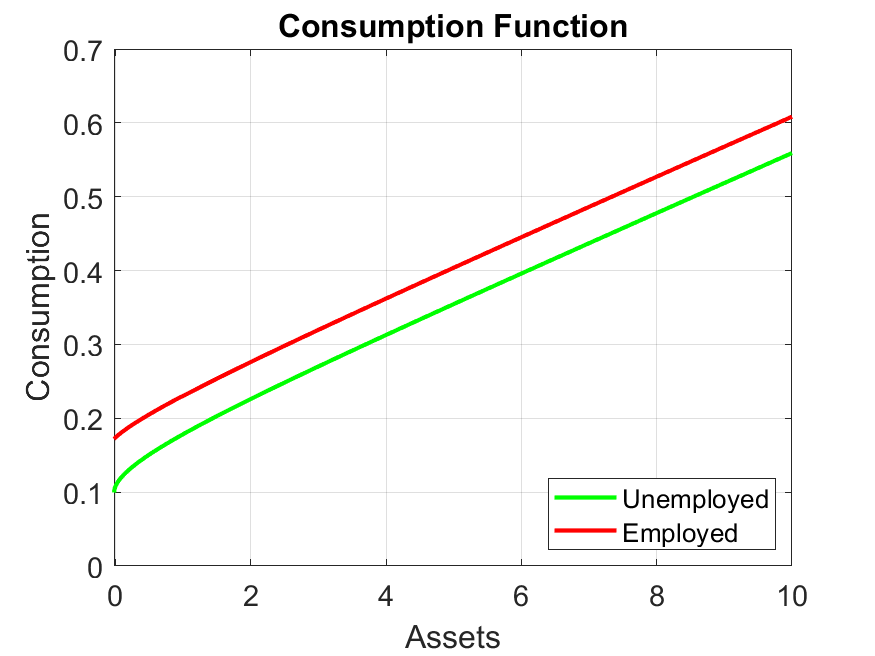
\includegraphics[width=0.6\textwidth]{homework/Solutions/homework_3_coding/consumption_vs_assets.png}
\end{center}

\subsection*{Question 2}
The savings plot mirrors the consumption plot. The unemployed draw on savings for any positive value of assets, whereas the employed only start consuming their savings when assets are roughly larger than 1. That is, the employed save part of their income for assets lower than 1. Again, the gap between the groups is fairly constant after the first asset unit.\\
\begin{center}
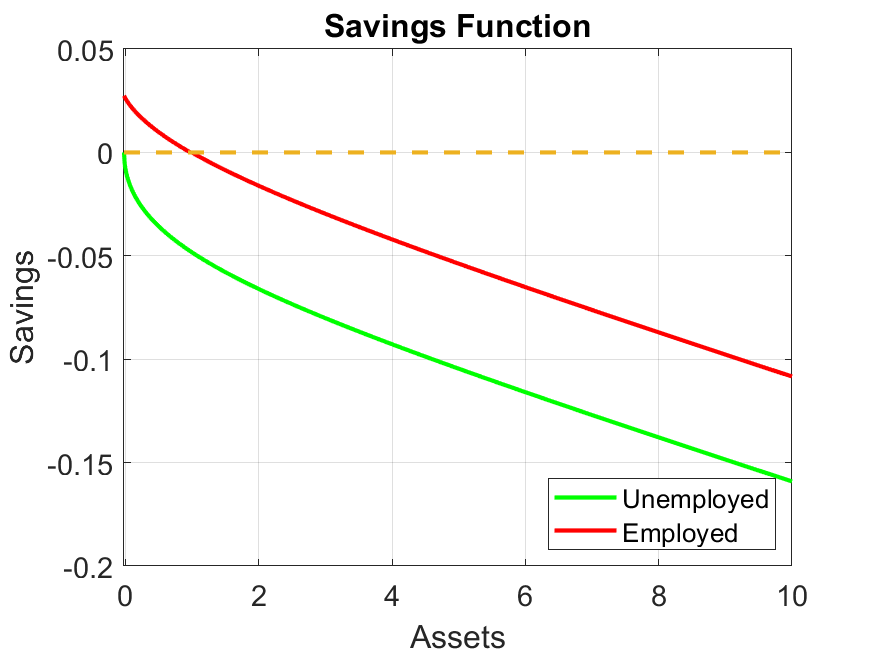
\includegraphics[width=0.6\textwidth]{homework/Solutions/homework_3_coding/savings_vs_assets.png}
\end{center}

\subsection*{Question 3}
The value function is negative since the coefficient of relative risk aversion is larger than 1 (which makes the CRRA utility lower than 0). The value function of the employed is naturally always larger than that of the unemployed, but the value functions converge as asset levels increase. This happens because even though the gap in consumption between the two groups is fairly constant, the marginal utility of the extra unit of consumption is lower. Therefore, as $a$ goes to infinity, present consumption/income ceases to matter.\\
\begin{center}
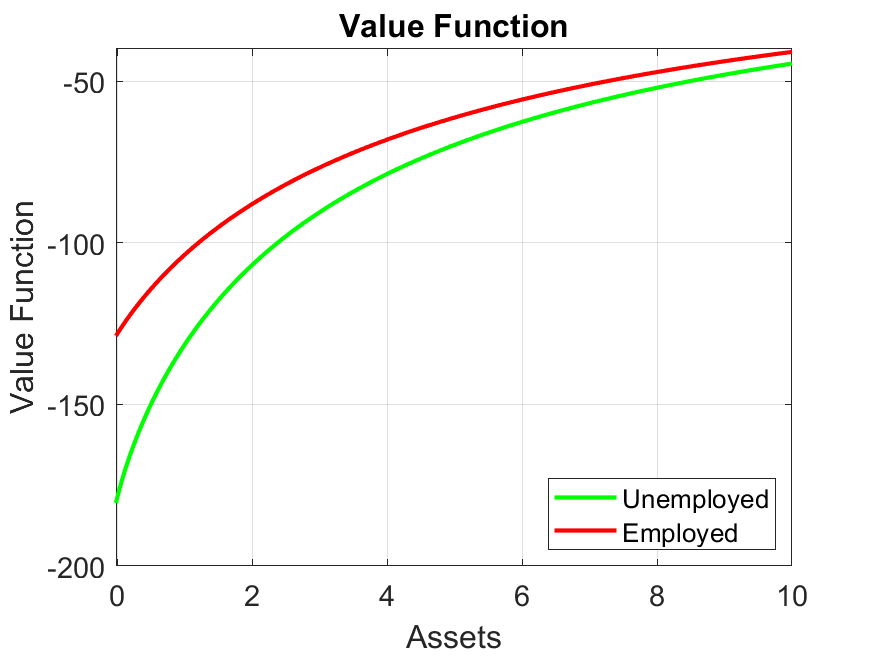
\includegraphics[width=0.6\textwidth]{homework/Solutions/homework_3_coding/value_function_vs_assets.png}
\end{center}

\subsection*{Question 4}
The Huggett model helps explain the existence and persistence of income and wealth inequality in an economy. Since agents face uninsurable idiosyncratic risk (e.g., job loss or income fluctuations), they end up with different levels of wealth, depending on their income trajectories and savings behavior.\\
Note also that in the Hugget model, wealth allows for better consumption smoothing, reducing fluctuations in utility across different states of employment. In the aggregate, economies with higher average wealth are likely to experience less volatility in consumption, especially during economic downturns. Due to uninsurable risk (the lower bound in $a$), however, households may engage in precautionary savings — i.e. saving more to guard against potential adverse income shocks. This suggests a role for the state to make use of policies that insure against these risks (e.g. unemployment insurance).\\


\subsection*{Code}
\lstset{
    language=Matlab,
    basicstyle=\ttfamily\small,
    keywordstyle=\color{blue},
    commentstyle=\color{green!50!black},
    stringstyle=\color{red},
    numbers=left,
    numberstyle=\tiny,
    stepnumber=1,
    numbersep=5pt,
    backgroundcolor=\color{white},
    tabsize=4,
    showspaces=false,
    showstringspaces=false,
    breaklines=true,
    breakatwhitespace=true,
    frame=single,
    captionpos=b
}

\begin{lstlisting}
clear all;
close all;

% Parameters
risk_aversion = 2; % CRRA utility with parameter risk_aversion
interest_rate = 0.03; 
discount_rate = 0.05;
income_unemployed = 0.1;
income_employed = 0.2;
income = [income_unemployed, income_employed];
lambda_unemployed = 0.02;
lambda_employed = 0.03;
lambda = [lambda_unemployed, lambda_employed];
asset_min = -0.02; % borrowing constraint
asset_max = 2;
num_points = 1000;
assets = linspace(asset_min, asset_max, num_points)';
delta_asset = (asset_max - asset_min) / (num_points - 1);
assets_matrix = [assets, assets];
income_matrix = ones(num_points, 1) * income;

max_iterations = 1000;
time_step = 1000;
convergence_criterion = 1e-6;

% Initialize matrices for forward and backward differences
dV_forward = zeros(num_points, 2);
dV_backward = zeros(num_points, 2);
consumption = zeros(num_points, 2);

% Transition matrix for switching between employment states
transition_matrix = [-speye(num_points) * lambda(1), speye(num_points) * lambda(1); 
                     speye(num_points) * lambda(2), -speye(num_points) * lambda(2)];

% Initial guess for the value function
value_function_initial(:, 1) = (income(1) + interest_rate .* assets).^(1 - risk_aversion) / (1 - risk_aversion) / discount_rate;
value_function_initial(:, 2) = (income(2) + interest_rate .* assets).^(1 - risk_aversion) / (1 - risk_aversion) / discount_rate;
value_function = value_function_initial;

for iteration = 1:max_iterations
    V = value_function;
    V_history(:, :, iteration) = V;
    
    % Backward difference
    dV_backward(2:num_points, :) = (V(2:num_points, :) - V(1:num_points-1, :)) / delta_asset;
    dV_backward(1, :) = (income + interest_rate .* asset_min).^(-risk_aversion); % Boundary condition at asset_min

    % Forward difference
    dV_forward(1:num_points-1, :) = (V(2:num_points, :) - V(1:num_points-1, :)) / delta_asset;
    dV_forward(num_points, :) = (income + interest_rate .* asset_max).^(-risk_aversion); % Boundary condition at asset_max
    
    % Consumption and savings with backward difference
    consumption_backward = dV_backward.^(-1 / risk_aversion);
    savings_backward = income_matrix + interest_rate .* assets_matrix - consumption_backward;

    % Consumption and savings with forward difference
    consumption_forward = dV_forward.^(-1 / risk_aversion);
    savings_forward = income_matrix + interest_rate .* assets_matrix - consumption_forward;
    
    % Consumption and derivative of value function at steady state
    consumption_steady = income_matrix + interest_rate .* assets_matrix;
    dV_steady = consumption_steady.^(-risk_aversion);
    
    % Upwind scheme for choosing forward or backward differences
    use_forward = savings_forward > 0;
    use_backward = savings_backward < 0;
    use_steady = (1 - use_forward - use_backward);
    
    dV_upwind = dV_forward .* use_forward + dV_backward .* use_backward + dV_steady .* use_steady;
    consumption = dV_upwind.^(-1 / risk_aversion);
    utility = consumption.^(1 - risk_aversion) / (1 - risk_aversion);
    
    % Construct matrix for the linear system
    X = -min(savings_backward, 0) / delta_asset;
    Y = -max(savings_forward, 0) / delta_asset + min(savings_backward, 0) / delta_asset;
    Z = max(savings_forward, 0) / delta_asset;
    
    A1 = spdiags(Y(:, 1), 0, num_points, num_points) + spdiags(X(2:num_points, 1), -1, num_points, num_points) + spdiags([0; Z(1:num_points-1, 1)], 1, num_points, num_points);
    A2 = spdiags(Y(:, 2), 0, num_points, num_points) + spdiags(X(2:num_points, 2), -1, num_points, num_points) + spdiags([0; Z(1:num_points-1, 2)], 1, num_points, num_points);
    A = [A1, sparse(num_points, num_points); sparse(num_points, num_points), A2] + transition_matrix;
    
    B = (discount_rate + 1 / time_step) * speye(2 * num_points) - A;
    
    utility_stacked = [utility(:, 1); utility(:, 2)];
    V_stacked = [V(:, 1); V(:, 2)];
    
    b = utility_stacked + V_stacked / time_step;
    V_stacked = B \ b; % Solve system of equations
    
    V = [V_stacked(1:num_points), V_stacked(num_points+1:2*num_points)];
    
    V_change = V - value_function;
    value_function = V;
    
    if max(max(abs(V_change))) < convergence_criterion
        disp('Value Function Converged, Iteration = ')
        disp(iteration)
        break
    end
end

savings = income_matrix + interest_rate .* assets_matrix - consumption;

%change working directory to the folder where this script is located
cd(fileparts(which(mfilename)));

figure;
plot(assets, consumption(:, 1), 'g', 'LineWidth', 2); hold on;
plot(assets, consumption(:, 2), 'r', 'LineWidth', 2);
grid on;
xlabel('Assets');
ylabel('Consumption');
xlim([asset_min asset_max]);
title('Consumption Function');
legend('Unemployed', 'Employed', 'Location', 'southeast');
set(gca, 'FontSize', 14);
%save the image in the main folder, call it consumption_vs_assets
saveas(gcf, 'consumption_vs_assets.png');

figure;
plot(assets, savings(:, 1), 'g', 'LineWidth', 2); hold on;
plot(assets, savings(:, 2), 'r', 'LineWidth', 2);
plot(assets, zeros(num_points, 1), '--', 'LineWidth', 2);
grid on;
xlabel('Assets');
ylabel('Savings');
xlim([asset_min asset_max]);
title('Savings Function');
legend('Unemployed', 'Employed', 'Location', 'southeast');
set(gca, 'FontSize', 14);
%save the image in the main folder, call it savings_vs_assets
saveas(gcf, 'savings_vs_assets.png');

figure;
plot(assets, V(:, 1), 'g', 'LineWidth', 2); hold on;
plot(assets, V(:, 2), 'r', 'LineWidth', 2);
grid on;
xlabel('Assets');
ylabel('Value Function');
xlim([asset_min asset_max]);
title('Value Function');
legend('Unemployed', 'Employed', 'Location', 'southeast');
set(gca, 'FontSize', 14);
%save the image in the main folder, call it value_function_vs_assets
saveas(gcf, 'value_function_vs_assets.png');
\end{lstlisting}


\end{document}

